\chapter{Background Reading}
\label{chap:background-reading}

\section{Synote}
\label{sec:synote}

\subsection{Conventions}
\label{subsec:conventions}

Every developer has their own programming style. When numerous individuals are contributing to a software product over time, it is necessary to provide a contribution document to ensure all developers adhere to the same conventions. Synote's conventions that applied to our development were:

\begin{itemize}
    \item \textbf{Promises over Callbacks} - To make the asynchronous code easier to read and understand.
    \item \textbf{Specific error structure} - A JSON with properties for the thrown error and an appropriate error message.
    \item \textbf{HTML element IDs} - All elements must have an \texttt{id} attribute of the form  \texttt{$<$name$>$\_$<$type$>$} where \texttt{name} is an intuitive name for the element and \texttt{type} corresponds to the type of the element. 
    \item \textbf{Server side testing} - Trigger all branches. If a branch cannot be tested it is considered a bug.\\ 
\end{itemize}

There are several additional conventions found in \texttt{CONTRIBUTING.md} which is a continuously evolving document. New conventions have been introduced as a result of our development, such as the HTML element ID convention and conventions regarding server side testing, which are discussed in \textbf{Chapter \ref{chap:further-work}}.  

\section{Payment Systems}
\label{sec:payment-systems}

% Should probably have nomenclature section to define: Merchant, Payment Gateway, Payment Processor, Merchant Account

\subsection{Introduction}
\label{sec:payment-intro}

E-Commerce has existed in various forms since the 1970s with its seminal act being a drug deal between Stanford and MIT students \cite{power-mike-online-highs}. Later that same decade Michael Aldrich demonstrated the first online shopping system. This system was used in 1984 for the first time to buy groceries from Tesco, marking the first true Business-To-Customer online transaction \cite{winterman-kelly-online-shopper}. Since Sir Tim Berners-Lee invented the World Wide Web, E-Commerce has grown substantially with industry revenue in the UK reaching \euro{157 billion} in 2016 \cite{khaksar-2016}.\\

The primary component of E-Commerce is the online payment system. A common approach for such systems is: Merchants collect payment information from customers, then send the information through a payment gateway to a payment processor which in turn pays into a merchant account. The way in which merchants collect payment information is an important concern which is handled in one of the several ways discussed in \textbf{Section \ref{subsec:gathering-payment-data}}.

\subsection{Considerations}
\label{subsec:considerations}

Security is an essential consideration for online payment systems. E-Commerce begins with customers trusting that the system provided by a merchant is \textit{safe} to use. For an online transaction to be considered \textit{safe}, it must be:

\begin{itemize}
	  \item Confidential - Inaccessible to unauthorized parties.
    \item Encrypted - Only decrypted by an authorized party.
    \item Auditable - Recorded to compliant standard.
    \item Non-Repudiable - Undeniable by both sender and recipient.
    \item Authenticated - Access controlled through an authentication mechanism.
    \item of Integrity - Unalterable during transmission.
\end{itemize}

The Payment Card Industry (PCI) Security Standards Council, exists to develop standards which ensure the above criteria are met. The Data Security Standard (DSS) created by the PCI council "provides a baseline of technical and operational requirements designed to protect account data" and "applies to \textit{\textbf{all}} entities involved in payment card processing--including merchants" \cite{PCI-DSS}.\\

PCI DSS is intended to protect cardholder data that is "processed, stored or transmitted by merchants" \cite{PCI-DSS}. The forms of data in question are depicted in \textbf{Figure \ref{fig:card-data}}, each of which have guidelines associated with them regarding storage and protection. Payment gateway services handle most PCI DSS compliance to remove the burden from the merchant but in some cases, not all of it, as described in \textbf{Section \ref{subsec:gathering-payment-data}}.

\begin{figure}[!hbt]
  	\centering
 	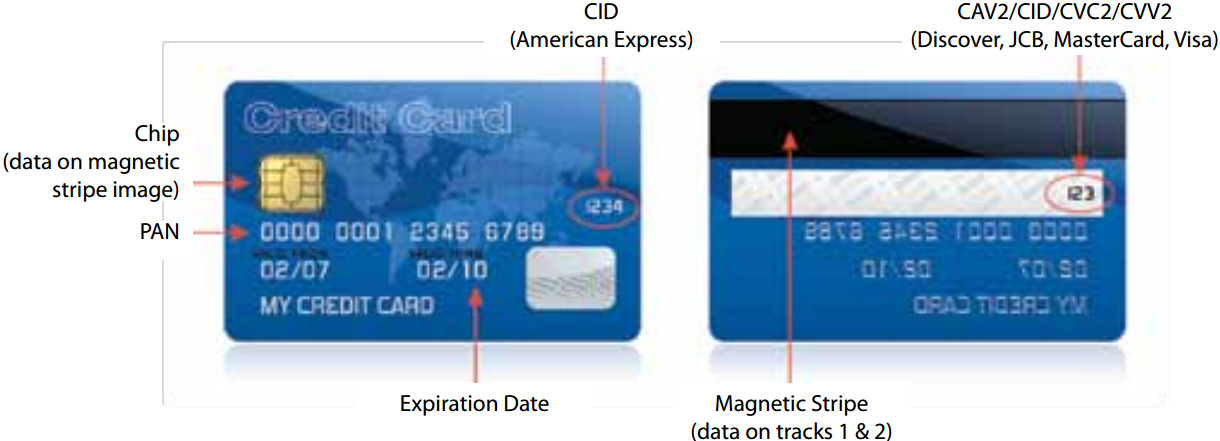
\includegraphics[width=\textwidth]{card-data.png}
  	\caption{Types of Data on a Payment Card\cite{card-data}}
 	\label{fig:card-data}
\end{figure}

\subsubsection{Security}
\label{subsec:security}

Encryption is an essential security measure when transmitting payment information over a network and ensures that only a specified receiver can decrypt the information. PCI DSS dictates the use of Hypertext Transfer Protocol Secure (HTTPS) which use either Secure Sockets Layer (SSL) or Transport Layer Security (TLS) protocols that have an asymmetric Public Key Infrastructure (PKI) system. This means that information can be encrypted with one key at the sender and decrypted by a different key at the receiver or vice-versa \cite{comodo}.\\

To establish a secure connection over HTTPS, an HTTPS/SSL certificate is required, which creates a binding between an organizational identity and a domain name, server name or host name \cite{ssl-certificate}. This certificate is used during a handshake procedure between sender and receiver to establish a secure connection through which payment data may be sent.

\subsection{Gathering Payment Data}
\label{subsec:gathering-payment-data}

The process of collecting a customer's payment information differs between payment gateway providers. The three main methods include:

\begin{enumerate}
	\item Redirection to payment website
    \item Form generated by payment gateway provider
    \item Custom form provided by merchant
\end{enumerate}

Methods 1 \& 2 fully remove the burden of PCI DSS compliance from the merchant as both circumvent processing, storage and transmission on/through the merchants web service. Method 3 however, involves the merchant collecting the payment information, potentially performing validation on the input and sending the information to the payment gateway. It is important to distinguish at this time that the payment information is merely being handled on a client and not sent through the merchants server. To remain compliant with this method, the data has to be encrypted and sent directly through a secure connection to the payment gateway, where it can be tokenized. Such tokens can be processed and stored on a merchant's server in a compliant manner. A collection of payment gateway services and their supported data gathering methods are shown in \textbf{Table \ref{tab:gateway-providers}}. \\

\begin{center}
\begin{tabular}{ |p{3.5cm}|p{1.75cm}|p{2cm}|p{2cm}|  }
 \hline
 	\multicolumn{4}{|c|}{Payment Gateway Services Data Gathering Methods} \\
 \hline
 	\multicolumn{1}{|c|}{Provider} &
 	\multicolumn{1}{|c|}{Redirection} &
 	\multicolumn{1}{|c|}{Generated Form} &
 	\multicolumn{1}{|c|}{Merchant Form}  \\
 \hline
 	Authorize.Net\cite{authorize-net} & \multicolumn{1}{|c|}{Yes} & \multicolumn{1}{|c|}{No} & \multicolumn{1}{|c|}{Yes} \\
 \hline
 	PayPal\cite{paypal} & \multicolumn{1}{|c|}{Yes} & \multicolumn{1}{|c|}{Yes} & \multicolumn{1}{|c|}{Yes (Pro)} \\
 \hline
 	amazon payments\cite{amazon-payments} & \multicolumn{1}{|c|}{Yes} & \multicolumn{1}{|c|}{No} & \multicolumn{1}{|c|}{No} \\
 \hline
    Stripe\cite{stripe} & \multicolumn{1}{|c|}{Yes} & \multicolumn{1}{|c|}{Yes} & \multicolumn{1}{|c|}{Yes} \\
 \hline
 	Braintree (PayPal)\cite{braintree} & \multicolumn{1}{|c|}{Yes} & \multicolumn{1}{|c|}{No} & \multicolumn{1}{|c|}{No} \\
 \hline
\end{tabular}
\captionof{table}{Payment Gateway Providers}
\label{tab:gateway-providers}
\vspace{0.4cm}
\end{center}

\section{Frameworks}
\label{sec:frameworks}

\section{Testing}
\label{sec:testing}

\section{JavaScript Test Frameworks}
\label{sec:frameworks}

\section{QA Process}
\label{sec:qa-process}
